\begin{frame}
    \frametitle{Parallelization scheme}
    \framesubtitle{$j-$parallelization scheme}

    Our configuration is based in the idea presented in~\cite{NitadoriAarseth2012},

    \begin{center}
    \begin{figure}[H]
        \centering
    \colorbox{white}{
        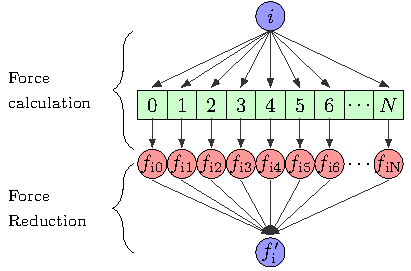
\includegraphics[width=0.55\textwidth]{img/force_split_reduction.pdf}
    }
        \caption{Parallelization scheme to split the $j-$loop instead of the $i-$loop.
                 In this case, we have two sections, the first is to calculate
                 the force interactions of the $i-$particle with the whole
                 system but by different threads. Then a reduction (sum) is necessary
                 to get the new value for the $i-$particle force.}
        \label{fig:force_split_reduction}
    \end{figure}
    \end{center}

\end{frame}

\begin{frame}
    \frametitle{Implementation}
    \framesubtitle{Class diagram}
    \begin{center}
        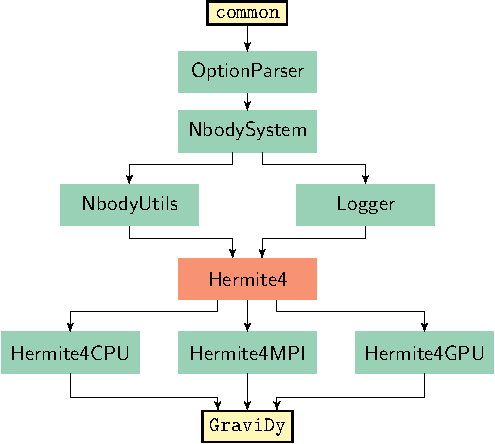
\includegraphics[height=0.8\textheight]{img/files_structure.pdf}
    \end{center}
\end{frame}

